\chapter{Architecture}

\section{High Level View}
\begin{center}
\begin{figure}
  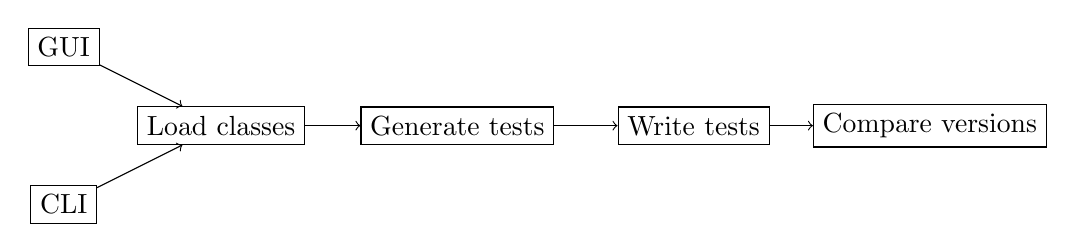
\begin{tikzpicture}
    \coordinate(origin);
    \node(core) at (origin) [draw] {Generate tests};
    \node(control) at ([left=3cm] core) [draw] {Load classes};
    \node(output) at ([right=3cm] core) [draw] {Write tests};
    \node(compare) at ([right=3cm] output) [draw] {Compare versions};
    \node(gui) at ([left=2cm,above=1cm] control) [draw] {GUI};
    \node(cli) at ([left=2cm,below=1cm] control) [draw] {CLI};

    \draw[->] (control) -> (core);
    \draw[->] (core) -> (output);
    \draw[->] (output) -> (compare);
    \draw[->] (gui) -> (control);
    \draw[->] (cli) -> (control);
  \end{tikzpicture}
\caption{A short summary of the control flow of SpLATS}
\label{fig:Architecture_HighLevel}
\end{figure}
\end{center}

  Figure \ref{fig:Architecture_HighLevel} shows the overall view of the system. There is a test generator, an output module, a wrapper to control the two, and either a graphical or command-line interface to control that.

    There's an inner core that generates the tests, an outer layer that controls it and handles file input and output, and a wrapper to pass options to the outer layer. These sections are explained in more detail in the following section.
    
\section{Lower Level Architecture}

  \begin{center}
  \begin{figure}
  
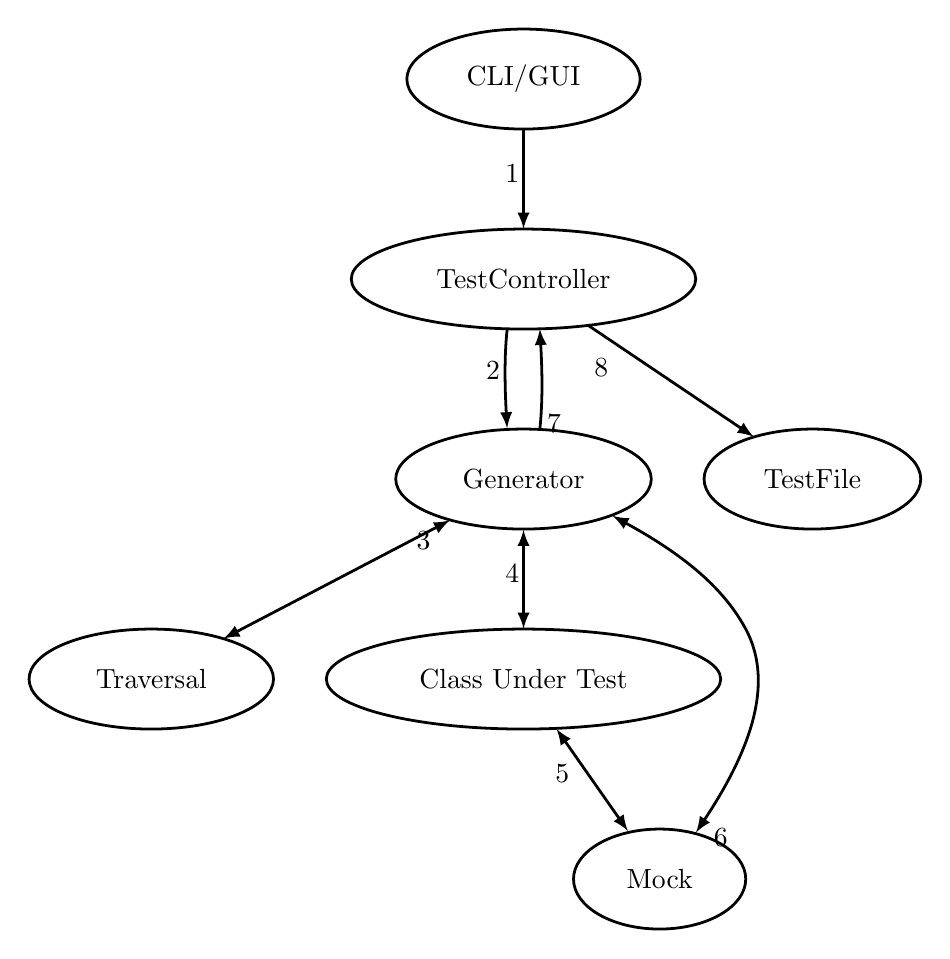
\begin{tikzpicture}[>=latex,line join=bevel,]
  \pgfsetlinewidth{1bp}
%%
\pgfsetcolor{black}
  % Edge: Generator -> TestController
  \draw [->] (183.91bp,180.28bp) .. controls (184.71bp,188.03bp) and (184.94bp,197.36bp)  .. (183.88bp,216.05bp);
  \definecolor{strokecol}{rgb}{0.0,0.0,0.0};
  \pgfsetstrokecolor{strokecol}
  \draw (189bp,182bp) node {7};
  % Edge: TestController -> TestFile
  \draw [->] (201.34bp,217.29bp) .. controls (216.4bp,207.16bp) and (236.12bp,193.88bp)  .. (260.86bp,177.23bp);
  \draw (206bp,202bp) node {8};
  % Edge: Class Under Test -> Mock
  \draw [<->] (189.86bp,72.055bp) .. controls (200.24bp,57.222bp) and (205.14bp,50.222bp)  .. (215.59bp,35.307bp);
  \draw (192bp,56bp) node {5};
  % Edge: CLI/GUI -> TestController
  \draw [->] (178bp,287.7bp) .. controls (178bp,279.98bp) and (178bp,270.71bp)  .. (178bp,252.1bp);
  \draw (174bp,272bp) node {1};
  % Edge: TestController -> Generator
  \draw [->] (172.12bp,216.05bp) .. controls (171.3bp,208.35bp) and (171.06bp,199.03bp)  .. (172.09bp,180.28bp);
  \draw (167bp,201bp) node {2};
  % Edge: Generator -> Class Under Test
  \draw [<->] (178bp,143.7bp) .. controls (178bp,128.69bp) and (178bp,123.49bp)  .. (178bp,108.1bp);
  \draw (174bp,128bp) node {4};
  % Edge: Generator -> Traversal
  \draw [<->] (151.53bp,147.17bp) .. controls (122.82bp,132.17bp) and (98.445bp,119.44bp)  .. (69.963bp,104.56bp);
  \draw (142bp,140bp) node {3};
  % Edge: Mock -> Generator
  \draw [<->] (240.08bp,34.735bp) .. controls (257.89bp,61.544bp) and (269.18bp,87.189bp)  .. (258bp,108bp) .. controls (249.58bp,123.68bp) and (234.26bp,135.5bp)  .. (210.02bp,148.79bp);
  \draw (249bp,33bp) node {6};
  % Node: CLI/GUI
\begin{scope}
  \definecolor{strokecol}{rgb}{0.0,0.0,0.0};
  \pgfsetstrokecolor{strokecol}
  \draw (178bp,306bp) ellipse (42bp and 18bp);
  \draw (178bp,306bp) node {CLI/GUI};
\end{scope}
  % Node: Generator
\begin{scope}
  \definecolor{strokecol}{rgb}{0.0,0.0,0.0};
  \pgfsetstrokecolor{strokecol}
  \draw (178bp,162bp) ellipse (46bp and 18bp);
  \draw (178bp,162bp) node {Generator};
\end{scope}
  % Node: Class Under Test
\begin{scope}
  \definecolor{strokecol}{rgb}{0.0,0.0,0.0};
  \pgfsetstrokecolor{strokecol}
  \draw (178bp,90bp) ellipse (71bp and 18bp);
  \draw (178bp,90bp) node {Class Under Test};
\end{scope}
  % Node: Traversal
\begin{scope}
  \definecolor{strokecol}{rgb}{0.0,0.0,0.0};
  \pgfsetstrokecolor{strokecol}
  \draw (44bp,90bp) ellipse (44bp and 18bp);
  \draw (44bp,90bp) node {Traversal};
\end{scope}
  % Node: TestController
\begin{scope}
  \definecolor{strokecol}{rgb}{0.0,0.0,0.0};
  \pgfsetstrokecolor{strokecol}
  \draw (178bp,234bp) ellipse (62bp and 18bp);
  \draw (178bp,234bp) node {TestController};
\end{scope}
  % Node: TestFile
\begin{scope}
  \definecolor{strokecol}{rgb}{0.0,0.0,0.0};
  \pgfsetstrokecolor{strokecol}
  \draw (282bp,162bp) ellipse (39bp and 18bp);
  \draw (282bp,162bp) node {TestFile};
\end{scope}
  % Node: Mock
\begin{scope}
  \definecolor{strokecol}{rgb}{0.0,0.0,0.0};
  \pgfsetstrokecolor{strokecol}
  \draw (227bp,18bp) ellipse (31bp and 18bp);
  \draw (227bp,18bp) node {Mock};
\end{scope}
%
\end{tikzpicture}


  \caption{A more in-depth summary of the control flow of SpLATS}
  \label{fig:Architecture_LowLevel}
  \end{figure}
  \end{center}
  Figure ~\ref{fig:Architecture_LowLevel} shows the workflow at a more in-depth level.
  \begin{enumerate}
  \small
  \item The user starts a UI of their choice, and passes in the file or files to be tested, a directory to put the finished tests, a traversal method and any parameters for that method.
    The interface then starts the TestController, which creates the output directory if one is needed, and loads the input files and their relevant classes.
  \item The TestController then initializes a Generator for each class, with the traversal method and parameters.
  \item The Generator talks to the traversal method.
  \item The traversal method responds to the Generator.
  \item Every Test produced by the Generator is sent to the TestController.
  \item The Tests are sent to TestFile, which wraps the tests with the necessary code to be run by Ruby's Test::Unit framework.
  \end{enumerate}
  
  \subsection{User Interface}
  \setcounter{secnumdepth}{4}
  \subsubsection{Command Line Interface}
  \subsubsection{Graphical User Interface (GUI)}
  \paragraph{Choice of framework}
  The GUI was initially implemented with a stand-alone Ruby program Shoes\footnote{\url{http://shoesrb.com/}}. This came shipped with its own version of Ruby. After some discussion, it was decided that we should try to use as many Gems\footnote{Ruby's equivalent of libraries} as possible, rather than stand-alone programs which the user must install. For this reason, the GUI was ported over to Green Shoes\footnote{\url{https://github.com/ashbb/green_shoes}} which can be installed by the standard "gem install" command, loaded in SpLATS by "require green\_shoes" and run as a normal Ruby file.
  
  \paragraph{Design}
  The GUI was designed to be minimalist with as few buttons as possible. As no one in the group would proclaim to be a designer, the look of the GUI is minimalist as well. The images are used to illustrate the workflow the user goes through when first loading the GUI.
  
  Figure \ref{fig:GUI_Page1} shows the page the user sees when they first open the GUI. This gives them the option to load the version of the code to generate tests for. Before the file is loaded, the button saying "Load first version of the code" is all they see. There is no other information on the first page, because it is assumed that the user wants to just begin testing and they already know what the program does. The "file open" dialog will not allow the user to cancel, nor allow the user to select a file which isn't '.rb'. Once a valid file is loaded, the "next" button and the text box appear. The text box is there to show the user what the inside of the file looks like, just so they are certain that they have loaded the correct version to test. There is a bug in Green Shoes, where the scroll bar doesn't appear on these text boxes, however they are scrollable with the mouse. The issues encountered with Green Shoes will be discussed in the "Problems" section. In future implementations of SpLATS, it would be possible to make this file box editable and writeable, but that is not high on the list of priorities.
Figure \ref{fig:GUI_Page2} is the same as the first page, only for the second version of the code.
  
  \begin{figure}
    \centering
    \subfloat[Load version 1]{\label{fig:GUI_Page1}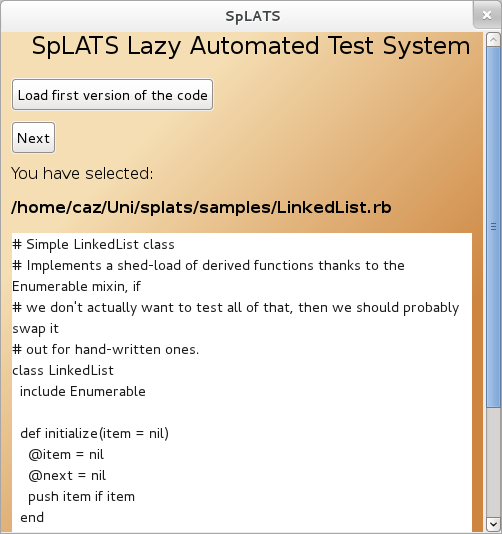
\includegraphics[width=0.4\textwidth]{page_1}}                
    \subfloat[Load version 2]{\label{fig:GUI_Page2}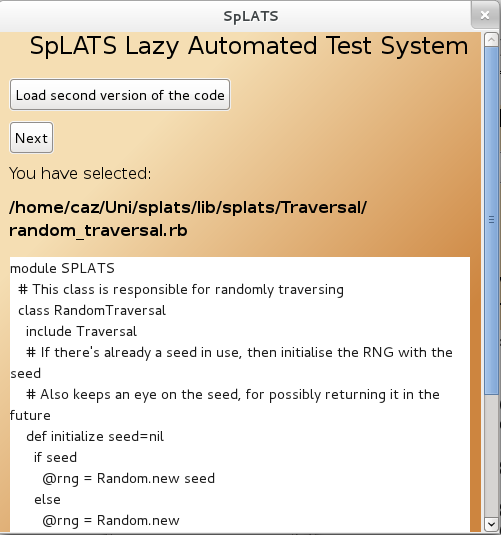
\includegraphics[width=0.4\textwidth]{page_2}}
    \caption{These pages are displayed when the user loads files to test}
    \label{fig:GUI_LoadVersions}
  \end{figure}
  
  Figure \ref{fig:GUI_Page3a} show the options the user then has to traverse the code. As discussed in the traversal methods, SpLATS currently only implements three traversal methods, but more can be added easily into the GUI. As the user changes their selection in the drop-down box, the options in the space below change to update inputs. Figures \ref{fig:GUI_Page3b} and \ref{fig:GUI_Page3c} illustrate this. The "next" button on third page doesn't do anything unless the extra parameters for "Random" and "Depth-Limited" are correct. Figure \ref{fig:GUI_Page3d} shows what the user sees when they've entered an invalid seed.
  
  \begin{figure}
    \centering
    \subfloat[Default traversal page]{\label{fig:GUI_Page3a}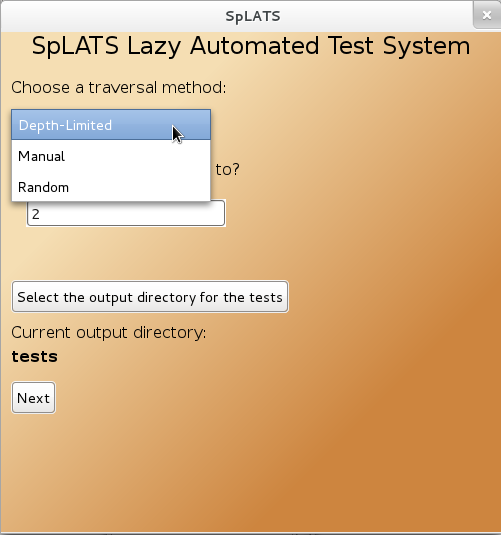
\includegraphics[width=0.4\textwidth]{page_3a}}
    \subfloat[Traversal options]{\label{fig:GUI_Page3b}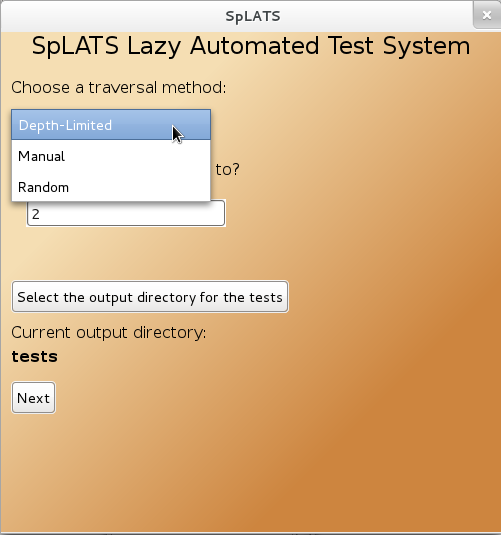
\includegraphics[width=0.4\textwidth]{page_3b}}
    \caption{The page the user sees when selecting a traversal method}
    \label{fig:GUI_SelectTraversal1}
  \end{figure}
  
  \begin{figure}
    \centering
    \subfloat[Random traversal]{\label{fig:GUI_Page3c}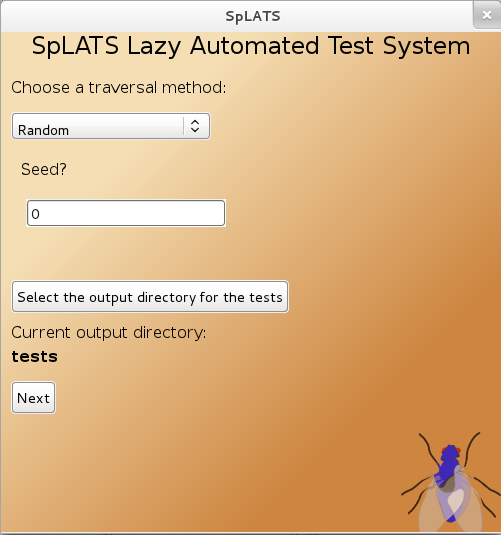
\includegraphics[width=0.4\textwidth]{page_3c}}
    \subfloat[Error in input]{\label{fig:GUI_Page3d}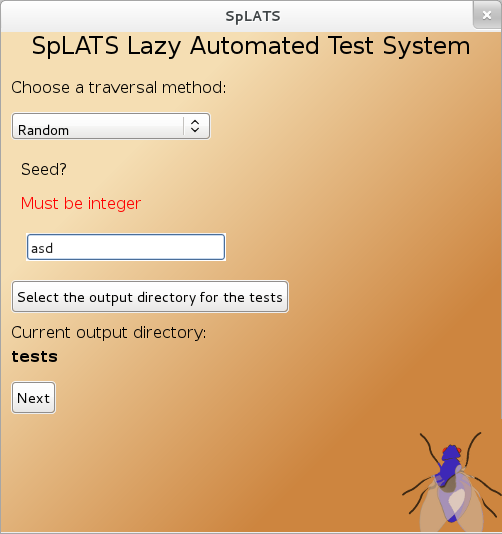
\includegraphics[width=0.4\textwidth]{page_3d}}
    \caption{Traversal page}
    \label{fig:GUI_SelectTraversal2}
  \end{figure}
  
  Once the user has input the correct information and they click "next", if they have selected "depth-limited" or "random" as the traversal methods, they will only see a page saying "generating tests", an alert pops up saying "testing complete" and SpLATS GUI will exit. It was decided not to draw graphs for these methods because the graphs will be extremely large.
  
  If the user has selected "Manual", then the GUI becomes more interesting. In order to have the GUI communicating with the code running SpLATS, threads were initially decided to be used. In theory, one thread would start the SpLATS process, and then when the user needed to give input, the thread would switch back to the GUI to ask for the user, the user would give input and so on until the end of the generation. The problem with threads is that they are determined by the thread scheduler, and it is difficult to time the threads and dictate exactly which thread should start when. This problem was overcome by using Ruby's in-built Fiber module. This is a much more lightweight implementation of Threads, but they don't need a scheduler, each Fiber has its own stack and the Fibers need to be specifically started and stopped. The three of these in combination were exactly what was needed to make the GUI run. Without the overhead of a scheduler, the GUI is extremely lightweight. The stack means that variables could be passed between Fibers, so the options available to the user are sent from the controller to the GUI, and the user's choice sent from the GUI to the controller. Figure \ref{fig:GUI_Page4a} shows the first choice the user will always have when in manual mode. They have to select which parameters to give to the initialise method (if there are any).
  
  \begin{figure}
    \centering
    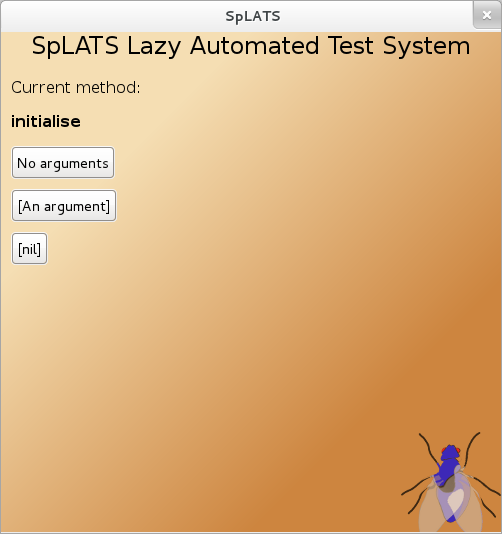
\includegraphics[width=0.5\textwidth]{page_4a}
    \caption{Manual traversal: "initialise" parameter choice}
    \label{fig:GUI_Page4a}
  \end{figure}
  
  \begin{figure}
    \centering
    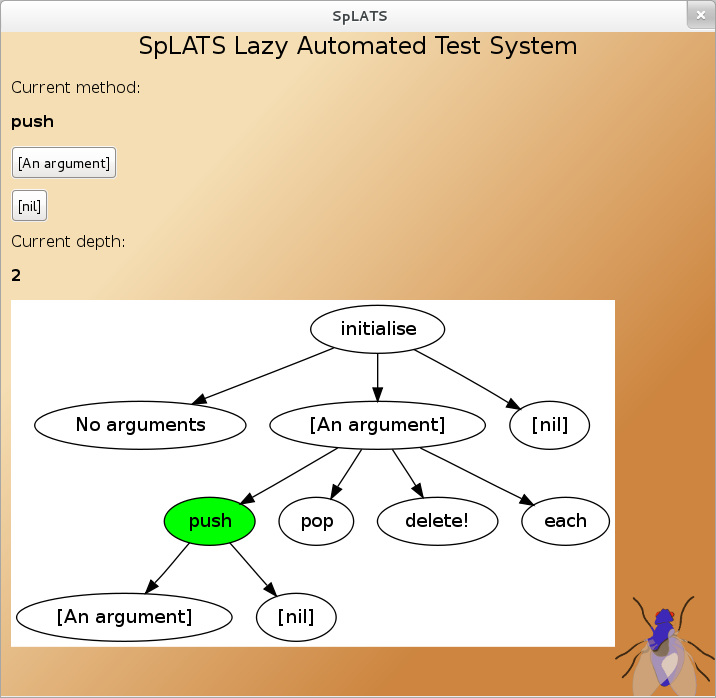
\includegraphics[width=0.8\textwidth]{page_4b}
    \caption{Manual traversal: "choose method" graph display of previous selections}
    \label{fig:GUI_Page4b}
  \end{figure}
  
  As the user steps down the traversal tree, they are presented a graph at each choice they have the option to make. This graph is generated from information stored in SpLATS as the user makes their selections. The graph was designed to be a maximum of three levels deep, because otherwise displaying the user the information becomes too cumbersome. Figure \ref{fig:GUI_Page4b} shows what the user sees when they have already made decisions, and they are being asked to select the next method to generate tests for. This way the user can keep track of the methods they have selected and at what depth they are currently at.

  \subsection{Output}
    When tests are generated by the Generator, they are added, line by line, to a Test object, which stores them in an internal representation called TestLine.
    This Test object is then passed to a TestFile, a wrapper around the built-in IO::File, which writes it to file.

    Initially, the Tests were stored until the Generator had finished, before being wrapped and output to a regular File.
    However, Tests store all the Mock objects associated with them, and thus this was changed so they could be garbage collected as soon as possible to reduce memory footprint.
    
    
